\documentclass[journal]{IEEEtran}

\usepackage{amsmath}
\usepackage{graphicx}

\begin{document}

\title{MOS Technology 6502 \\ Architecture, Design, and Impact}

\author{Chris~Ranc,~Travis~Whitaker}

\markboth{Journal of Computer Architecture Project Reports, May 2016}
{Journal of Computer Architecture Project Reports, May 2016}

\maketitle

\begin{abstract}
This report discusses the design and architecture of the MOS Technology 6502
CPU. The design of this CPU represents several key breakthroughs in
microprocessor design, and as a result its introduction significantly disrupted
extant markets and created entirely new applicational areas for microprocessor
products. The effects of this CPU's introduction are still observable today.
\end{abstract}

\begin{IEEEkeywords}
MOS Technology, Microprocessor, Computer Architecture
\end{IEEEkeywords}

\IEEEpeerreviewmaketitle

\section{Introduction}

\IEEEPARstart{T}{he} MOS Technology 6502, typically refered to as simply
``the sixty-five-oh-two,'' is an 8-bit microprocessor introduced in 1975. The
6502's design incorporated several architectural breakthroughs in microprocessor
design, allowing units to be sold at a small fraction of the cost of its
contemporary competitors, including the Motorola 6800, Intel 8080, and Zilog Z80
microprocessors. The 6502's low cost and power requirements are owed to its
small die size. Use of a statically scheduled instruction pipeline and simple
yet novel debugging features enabled the design to approach or even exceed the
throughput of its competitors while utilizing a fraction of the silicon. The low
unit cost and availability of cheap development boards for the 6502 spurred on
the home computer market in the early 1980's, and enabled the design of
affordable home video game consoles.

\section{History}

\subsection{Beginnings at Motorola}
Most of the engineers that designed the MOS 6502 originated from the team 
that developed the Motorola 6800 series.  Some of these engineers were John 
Buchanan the lead 6800 chip designer, Rod Orgill in charge of circuit analysis 
and chip layout (later worked on the 6501) [5], Bill Mensch who Designed 
peripheral IC's for the 6800 family, and Chuck Peddle Architectural Support of the 6800.
[2]  Designed the 6850 ACIA serial interface  and was the lead of architecture support 
for the 6502 [3]

Motorola target customers were large computing and electronics firms.
The main focus was to reduce development cost for these firms as opposed to 
reducing the cost of their processors.  Doing so by providsing prototype 
processors and providing development software through timesharing.  
Some of these target Firms were HP, Textronix, TRW, and Chrysler [4]

Chuck Peddle saw how clients disliked the high price of the 6800 (\$300) when 
accompanying sales representatives on customer visits. To remedy this Peddle and
other 6800 engineers who saw the issue began outlining a more cost effective design.
One that would remove inessential debugging features and utilize depletion-mode MOS 
transistors.  Doing so would reduce size to produce more chips on a silicon wafer and 
thus effectively reduce the cost to around \$25. [6]\newline

\centerline{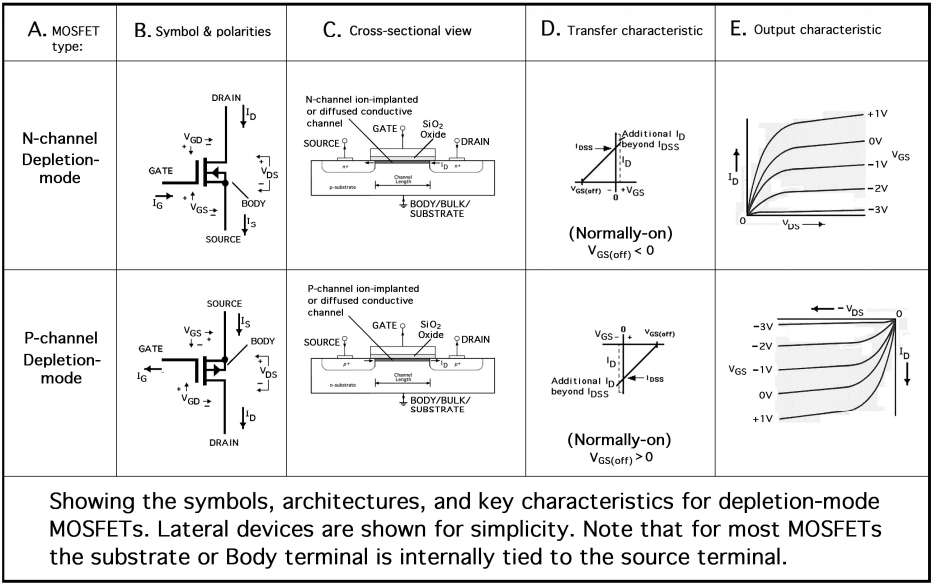
\includegraphics[scale=0.265]{images/Depletion_Mode_Table.png}}

\centerline{Depletion-Mode MOSFET Table [7]}

Due to Motorola's new fabrication plant in Austin Texas having difficulty with 
utilizing depletion-mode technology in fabrication and Motorola not liking the idea of designing 
cheaper processors Chuck Peddle's idea for making a more cost effective 6800 was dismissed.  
Peddle saw this as "product abandonment" so he decided to no longer work on the 6800 and 
move forward with his more effective design.  [6]

\subsection{Move to MOS Technology}
To continue his more ideal design for the 6800 Chuck Peddle teamed up with his old colleague John Pavinen 
from General Electric who was running a fabrication company by the name of MOS Technologies.  Bringing on
Bill Mensch and several other key Motorola engineers to this project they began work on Peddle's CPU .  
With MOS Technology they were able to better fabricate their designs with the use of depletion-mode MOS 
transistors.  Another key benefit of working with MOS Technologies was their improved fabrications process
that significantly reduced the production of defective chips.  Most fabrication methods in the 1970's 
had a 30\% success rate when producing chips.  MOS however developed a method in which a correction stage was 
added to the chip manufacturing process. It would attempt to remove errors before reaching the final 
fabrication stage which made the chip production success rate come to 70\% effectively reducing waste cost.  
To further improve cost effectiveness Peddle instructed his team to implement processor instructions that 
most customers required for their products.  Removing some of the more bloated debugging concepts that the 
Motorola 6800 had which in tandem with the use of depletion-mode technology significantly decreased the size
and ultimately cost of the processors. [6]  The end products being the MOS 6501 and 6502.   

\subsection{Motorola Lawsuit}
When their products were introduced to Wescon it became a massive hit.  Their low cost processor
received extensive press coverage which beneficial also had a downside.  Motorola was able to see the 
popularity of their former engineers work making them now a serious competitor.  At first they tried 
reducing the costs of their processors and design kits.  Their cost reduction didn't quite meet the cost of 
the MOS 6501 and 6502 so they they pursued an injunction in Federal Court to prevent MOS Technology from 
manufacturing and selling the chips.  

Motorola was able to push this through as they were a wealthy company with a believable case of infringement 
since many of their key engineers who designed the Motorola 6800 were also apart of the MOS 6502 and 6501 design
team.  Chuck Peddle, Bill Mensch, and a few other engineers were named as inventors in their patents for the
6800.  Along with this one of the engineers, Mike James, brought into project by Peddle took in his 6800
designs.[1]  Which Peddle had said not to do when they began work on the MOS 6501 and 6502.  Since MOS 
Technology was still small and lacked the money to fight this case they instead settled and agreed to 4
things.  MOS Technology would return the 6800 documents taken, pay Motorola \$200,000,  remove the 6501 from
their product line,  and agree to cross-license processor patents. [8]  This didn't affect the rise 
of the MOS Technology in the use of personal computers fortunately because the 6502 was their flagship processor 
while the 6501 was more of a demonstration model for their technology. [6]

\subsection{Beginnings of the Microcomputer}
With the legality troubles over MOS Technology began working on development kits to get their products out
to companies.  Chuck Peddle designed the MDT-650 (Microcomputer Development Terminal) which was a single 
board development computer with terminal. Another development board made that was sold partially completed 
was the KIM-1 (Keyboard Input Monitor) which was very popular amongst hobbyists as well as engineers. 
[6]

With the popularity of the MOS 6502 building it saw its first popular use by Apple Computers in the creation
of the Apple I developed by Steve Wozniak. The Apple II would also come to use the MOS 6502 but the biggest 
and most popular customer for the time to use the chip was Commodore in just about everyone of its products.  
Ranging from the Commodore PET, VIC-20, and the popular Commodore 64.  Even their floppy disk drive utilized 
a 6502 to function. This popular use lead to Commodore acquiring MOS Technology for developing their chips 
and giving them quicker access to newer chips.   Aside from the popularity of the processor in the personal 
computer market video games companies saw it as usable for creating processor based video games. [6]

\subsection{Home Game Consoles Emerge}
The Founders of Atari, Ted Dabney and Nolan Bushnell, in 1970's began to investigate microprocessor based 
video games as opposed to using discrete logic like for their arcade games.[9]  This would provide the ability 
to write games in software so a home entertainment system could play multiple different games.  Their 
prototype processor based console, titled Stella, utilized a lower cost version of the MOS 6502 called the 
6507.  The 6507 was basically a modified 6502 but cheaper to make for being a more ideal for its use in designing 
their prototype console.  This prototype Would com to be known as the Atari 2600.  


\subsection{Penetration in the Japanese Market}
Outside Atari the arcade market in japan caught hold of the chip and began utilizing a different variation of 
the 6502 made by Ricoh.  This variation removed binary-coded decimal and added 22 memory-mapped Registers for
sound, joystick reading, and sprite list DMA.  This modifed version of the 6502 was cost-effective and had more
features useful for video games.  However due to the obscurity of the 6502 in the Japanese market Nintendo had
to develop its own proprietary software development platform for making games.  The creation of which brought 
about the model for unified platform development as well as software liscensing that is still used today.[10]

\section{Implementation}

\subsection{Features and Specifications}

The 6502 is equipped with three 8-bit general purpose registers: an accumulator
A, and two index registers X and Y. The CPU also has
an 8-bit stack pointer a 16-bit program counter, and an 8-bit processor status
register. The 6502 utilizes a 16-bit memory address bus, however, none of the
general purpose registers available on the CPU are wide enough to accomodate a
whole memory address; this has interesting consequences for programming,
discussed in section IV.

Two interupt generating signals are provided, a maskable level sensitive
interrupt and a non-maskable edge sensitive interrupt. The non-maskable proved
critical for the design of game consoles, which must stop game logic during the
rendering of a frame for display on a television. Due to the limited memory
available on 6502-based systems, many game consoles would compute and buffer a
single scan line of the output image at once, rather than buffering the entire
frame. This rendering technique required only a small amount of memory, but
total use of the CPU throughout the frame rendering process was necessary. On
many 6502-based game consoles, the non-maskable interrupt was simply tied to the
60 Hz (America) or 50 Hz (Japan, Europe) vertical blanking synchronization
signal.

The original 6502 die used an 8 $\mu m$ process on a 3.9 x 4.3 mm die area,
embedded in a 40-pin ceramic DIP unit. Approximately 15\% of the area on the
original die was dedicated to the instruction decoding PLA. However, the PLA was
only mask-programmable, and there was effectively no way to update the
instruction decoding logic on the original 6502 chips. This would prove to be
problematic, as rushed development led to several quirks in the original
manufacturing run. The first very first lot of units shipped in 1975 exhibited
a bug in the ROR instruction, causing it to behave as a LSR
instruction without carry, and a bug in the JMP instruction when
performing an indirect jump. Several other batches and clones from other
manufacturers are known for various other strange quirks or undocumented
opcodes.

One of the most touted features of the Motorola 6800, the 6502's principal
competitor, was its extensive debugging facilities. The 6800 could be easily
halted with a non-maskable debugging interrupt, and the hardware even supported
something of a primitive core dump feature without the need for dual-port RAM.
The 6502 features only one built in debugging feature in contrast: a bus ready
signal. Exposing the bus ready signal was a simple enhancement, but proved
invaluable when debugging 6502 programs. A program under test could effectively
be ``stepped-through'' in hardware, by overriding the system clock with a
``step-through'' signal that may only be asserted when the bus ready signal
indicated the CPU was ready to move on to the next instruction. The 6502 was the
first affordable microprocessor with development boards featuring such a
hardware step-through feature, and this lone debugging facility proved
sufficient for the majority of 6502 program development.

\subsection{Typical System Configuration}

Contemporary 6502-based systems often features 1-2 MHz clock signals. Although
this is a small fraction of the clock frequency often used in systems based on
competing CPUs (e.g. the Motorola 68A70, a 6800 derivative, could operate at up
to 10 MHz), the 6502 pipeline allowed for similar throughputs to be achieved.
The control unit utilized both the rising edge and falling edge of the clock
signal for pipeline synchronization, allowing for partial overlap between
instruction fetch and execution.

The 6502 has a hard-wired memory map, so there is little variation in memory
architecture among 6502-based systems. Addresses 0100-01FF are reserved for the
stack, 4000-7FFF are reserved for memory-mapped IO components, and all addresses
FFF9 and up are reserved for the interrupt vector tables. Most early 6502-based
systems such as the Apple II, Commodore PET, and the Atari 2600 reserved
addresses 8000-FFF9 for program ROM. However, a technique known as bank
switching, first used on the Nintendo Famicom/NES, allowed using a portion of
this address space for indexing into one of several smaller memory banks. Care
had to be taken to reserve a critical code region for duplication on all banks,
otherwise program continuity would be impossible. This technique allowed
Famicom/NES games to approach several megabits in size; the largest licensed
game was \emph{Kirby's Adventure} with a 6 MBit ROM.

The memory-mapped IO region was critical for 6502-based home computers and game
consoles. Home computers and terminal-based development boards often used this
region for disk drives, tape drives, or printers. It was possible to use this
region for drawing video; the Commodore PET's video terminal operated this way.
However, only a small region of the framebuffer could be written out at a time,
so video terminals implemented with this technique often suffered from extremely
slow frame refresh rates. This was a concious trade-off made by Commodore for
the PET, as the system was designed strictly for the business market. Other
systems marketed for gaming, such as the Famicom/NES and the Commodore 64, used
dedicated video units with direct memory access to allow for a full frame to be
buffered for each television vertical blank synchronization. This freed CPU time
during rendering as well, as the CPU only had to initiate a DMA transfer for
each line of the frame. More advanced video effects could be accomplished, such
as dithering and transparency, by executing other memory operations during frame
drawing.

\section{Programming}

\subsection{Instruction Set}

The 6502 has 151 instructions. Instruction encoding is variable-width;
instructions vary from one to three bytes wide. Numerous variants and clones of
the 6502 were produced, and many of these units were not exactly compatible with
the original MOS Technology instruction set architecture. Perhaps the most
frequently omitted feature was the binary coded decimal mode. The BCD mode was
incorporated in the original design so that the 6502 could be positioned in the
calculator market. However, the 6502 saw limited use in this market sector and
even the earliest 6502 clones often omitted the BCD mode; a key example is the
Ricoh 2A03 used in the Nintendo Famicom/NES.

The 6502's limited registers and small stack size make programming in compiled
programming languages problematic. C compilers do exist for the architecture,
but went essentially unused in the production of commercial software. While most
commercial 6502 software is written in assembly language, interpreted languages
such as BASIC were also widely successful on the platform; notable examples
include the Apple II, Commodore PET, and Commodore 64, whose default ROMs all
booted into an integer BASIC interpreter.


\subsubsection{Arithmetic Instructions}

The 6502 supports addition with carry, subtraction with borrow, and bit-wise
operations. Arithmetic may only be performed on 8-bit operands, so operations on
wider quantities must be implemented by the programmer. The original MOS 6502
also had a binary coded decimal mode, activated by setting a bit in the program
status register. However, most ``compatible'' clones omited this mode.

Table \ref{arith} describes the arithmetic instructions available on the 6502.

\begin{table}
\centering
\begin{tabular}[H!]{|l|l|l|l|}
\hline
\textbf{Mnemonic} & \textbf{Description} & \textbf{Operand 1} \\
\hline
ADC & Add memory to A with carry. & M \\
AND & And memory with A. & M \\
ASL & Arithmetic shift left. & X,Y,A,M \\
BIT & Test bits in A with memory. & M \\
CMP & Compare A with memory. & M \\
CPX & Compare X with memory. & M \\
CPY & Compare Y with memory. & M \\
DEC & Decrement memory. & M \\
DEX & Decrement X. & \\
DEY & Decrement X. & \\
EOR & XOR A with memory. & M \\
INC & Incrememt memory. & M \\
INX & Incrememt X. & \\
INY & Increment Y. & \\
ORA & Or A with memory. & M \\
ROL & Rotate left. & A,M \\
ROR & Rotate right. & A,M \\
SBC & Subtract memory from A with borrow. & M \\
\hline
\end{tabular}
\caption{6502 Arithmetic Instruction}
\label{arith}
\end{table}

\subsubsection{Control Flow Instructions}

The 6502 features primitive support for subroutines with instructions that
automatically push/pop the program counter to/from the stack. However, the small
stack space made the effective use of coroutines critical to any non-trivial
6502 programs. Returning to the interrupted task from a interrupt handler is
also automatic; use of this functionality is required in the case of the
non-maskable interrupt, as the NMI pin will not be pulled high until the NMI
vector executes the RTI instruction.

Branch instructions accept an 8-bit relative offset to the current program
counter; longer jumps must be implemented with unconditional jumps or subroutine
calls.

Table \ref{control} describes the control flow instructions available on the
6502.

\begin{table}
\centering
\begin{tabular}[H!]{|l|l|l|l|}
\hline
\textbf{Mnemonic} & \textbf{Description} & \textbf{Operand 1} \\
\hline
BCC & Branch on carry clear. & M \\
BCS & Branch on carry set. & M \\
BEQ & Branch on zero set. & M \\
BMI & Branch on negative set. & M \\
BNE & Branch on zero clear. & M \\
BPL & Branch on negative clear. & M \\
BRK & Trigger maskable interrupt. & \\
BVC & Branch on overflow clear. & M \\
BVS & Branch on overflow set. & M \\
CLC & Clear carry. & \\
CLD & Clear decimal. & \\
CLI & Clear interrupt. & \\
CLV & Clear overflow. & \\
JMP & Unconditional jump. & M \\
JSR & Call subroutine. & M \\
NOP & No operation. & M \\
RTI & Return from interrupt handler. & \\
RTS & Return from subroutine. & \\
SEC & Set carry. & \\
SED & Set decimal. & \\
SEI & Set interrupt. & \\
\hline
\end{tabular}
\caption{6502 Control Flow Instructions}
\label{control}
\end{table}

\subsubsection{Memory Instructions}

The 6502 memory manipulation instructions operate only on 8-bit operands.
Notably, the accumulator is the only general purpose register that may be pushed
onto the stack. The 6502 does not have a strict subroutine calling convention,
but conventionally the A register is preserved by subroutine calls.

Table \ref{mem} describes the memory instructions available on the 6502.

\begin{table}
\centering
\begin{tabular}[H!]{|l|l|l|l|}
\hline
\textbf{Mnemonic} & \textbf{Description} & \textbf{Operand 1} \\
\hline
LDA & Load A with memory. & M \\
LDX & Load X with memory. & M \\
LDY & Load Y with memory. & M \\
PHA & Push A onto stack. & \\
PHP & Push status onto stack. & \\
PLA & Pull A from stack. & \\
PLP & Pull status from stack. & \\
STA & Store A in memory. & M \\
STX & Store X in memory. & M \\
STY & Store Y in memory. & M \\
TAX & Transfer A to X. & \\
TAY & Transfer A to Y. & \\
TSX & Transfer stack pointer to X. & \\
TXA & Transfer X to A. & \\
TXS & Transfer X to stack pointer. & \\
TYA & Transfer Y to A. & \\
\hline
\end{tabular}
\caption{6502 Memory Instructions}
\label{mem}
\end{table}

\subsection{Addressing Modes}

The 6502 is an 8-bit CPU in the truest sense; there aren't even any registers
capable of storing a full memory address. Naturally this has consequences for
performing memory operations. The 6502 features some unique addressing modes to
ease the process of pointer construction.

The expected addressing modes of immediate values, relative branches, and
absolute addressing are present; a full 16-bit literal address may be endoded
in pointer-accepting instructions. Absolute indexed addressing is also
supported; in this mode a 16-bit literal is added to the contents of the X or Y
registers to compute the final pointer.

Address construction difficulty arises when a full 16-bit address must be
computed at run-time. To aid this process, a specially designated address range
known as the ``zero page'' is provided. The zero page consists of the first 256
memory addresses (0000-00FF), and these addresses may be indexed by a single
byte literal. Zero page addresses may also be used for indirection, e.g.
``(\$AB,X)'' adds the contents of X to the zero page address \$AB, and
``(\$AB),Y'' adds the contents of Y to the value at the memory location at the
zero page address \$AB.

\subsection{Interrupts}

The 6502 features two programmable interrupts: an edge-triggered non-maskable
interrupt, and a level-triggered maskable interrupt. The maskable interrupt
is triggered by a high voltage on an open collector, or by execution of the
\emph{BRK} instruction, and jumps to address FFFE in the interrupt vector table.
The non-maskable interrupt is triggered by pulling the NMI line low. This
behavior may be leveraged by external components to detect when the NMI handler
is finished executing; the NMI is non-nestable, so the NMI signal won't be
pulled high again until the interrupt handler has returned. The NMI causes the
cpu to jump to address FFFA in the interrupt vector table.

Upon interrupt receipt, the CPU finishes the current instruction. Then the
program counter and program status registers are pushed onto the stack. The
program counter is then loaded with the address in the appropriate entry in the
interrupt vector table. The interrupt handler returns by executing the
RTI return from interrupt instruction. There are only 256 bytes
available on the 6502's stack, and each interrupt handler stack frame occupies
three such bytes. Therefore, it is critical that no deeply nested interrupt
handlers are executed on the 6502.

The 6502's reset signal also acts somewhat like a non-programmable interrupt.
After CPU start up is complete, the program counter is set to the address at
FFFC in the interrupt vector table. Typically this vector entry will contain
the address of the first byte of program ROM.

\section{Conclusion}

The MOS 6502 had a large impact on the microprocessor market. Its success
spurred on the home computer and home game console industries. This success is
largely owed to a number of cost and resource saving architectural innovations.
Its low cost had a permanent effect on the microprocessor industry; the cost of
its contemporary competitors, including the Motorola 6800 series, Intel 8080,
and Zilog Z80 fell substantially in subsequent generations. This market-wide
price depression effect, along with the availability of low cost development
hardware and home computer kits, is in part responsible for the home computer
revolution.

\begin{thebibliography}{1}

\bibitem{IEEEhowto:Bagnall}
Bagnall, Brian (2010). Commodore, a company on the edge. (2nd ed.). Winnipeg, Manitoba: Variant Press
\bibitem{IEEEhowto:Donohue}
Donohue, James F. (October 27, 1988). "The microprocessor first two decades: The way it was". EDN (Cahners Publishing) 
\bibitem{IEEEhowto:Hepworth}
Hepworth, Edward C., Rodney J. Means, Charles I. Peddle, "Asynchronous Communication Interface Adaptor", Patent 3975712, issued August 17, 1976
\bibitem{IEEEhowto:Motorola}
Motorola (August 5, 1976). "They stay out front with Motorola's M6800 Family". Electronics (McGraw-Hill) 49
\bibitem{IEEEhowto:}
"Motorola 6800 Oral History Panel" Thomas H. Bennett, John Ekiss, William (Bill) Lattin, Jeff Lavell. Computer History Museum, March 28, 2008, moderator: David Laws.
\bibitem{IEEEhowto:}
Matthews, Ian(2006), "The Leendary Chuck Peddle, Inventor of the Personal Computer",http://www.commodore.ca/commodore-history/the-legendary-chuck-peddle-inventor-of-the-personal-computer/
\bibitem{IEEEhowto:}
Harrison, Linden, "An Introduction to Depletion-Mode Mosfets"[pdf],http://www.aldinc.com/pdf/IntroDepletionModeMOSFET.pdf
\bibitem{IEEEhowto:}
"Motorola, MOS Technology settle patent suit". Electronics (New York: McGraw-Hill) 49 (7): 39. April 1, 1975
\bibitem{IEEEhowto:}
Chafkin, Max (April 1, 2009). "Nolan Busnell is Back in the Game". Inc.
\bibitem{IEEEhowto:}
Liedholm, Marcus; Liedholm, Mattias. "History of the Nintendo Entertainment System or Famicom". Nintendo Land
\bibitem{asm}
Leventhal, Lance A. \emph{6502 Assembly Language Programming}, 1986
\bibitem{isa}
\emph{Rockwell 6502 Programmers Reference}, 1981


\end{thebibliography}

\end{document}
